%% Copyright 2018 David Tolnay
%%
%% Licensed under the Apache License, Version 2.0 <LICENSE-APACHE or
%% http://www.apache.org/licenses/LICENSE-2.0> or the MIT license
%% <LICENSE-MIT or http://opensource.org/licenses/MIT>, at your
%% option. This file may not be copied, modified, or distributed
%% except according to those terms.
\documentclass[usepdftitle=false,aspectratio=169]{beamer}
\mode<presentation>{\usetheme{m}}

\usepackage{amssymb}
\usepackage{calc}
\usepackage{enumitem}
\usepackage{fancyvrb}
\usepackage{mathtools}
\usepackage{microtype}
\usepackage{pgfplots}
\usepackage{pifont}
\usepackage{scalefnt}
\usepackage{setspace}
\usepackage{ulem}
\usepackage{xspace}

\usepackage{tikz}
\usetikzlibrary{calc}
\usetikzlibrary{hobby}
\usetikzlibrary{patterns}
\usepgfplotslibrary{fillbetween}

\usepackage{minted}
\usemintedstyle{dtolnay}
\setminted{autogobble,xleftmargin=-.5em,escapeinside=~~}

\usepackage{scrextend}
\changefontsizes{15pt}

\newcommand{\plus}{\hspace{3pt}\raisebox{-.21em}{\scalefont{1.5}\Light+}\hspace{3pt}\xspace}
\title{Rust as TT sees it}
\author{dtolnay}
\date{}

\hypersetup{
  pdftitle={Rust as TT sees it},
  pdfauthor={David Tolnay},
  pdfsubject={Rust},
}

\definecolor{goldish}{HTML}{BD7A00}
\definecolor{greenish}{HTML}{008000}
\definecolor{tealish}{HTML}{147070}
\definecolor{redish}{HTML}{BA2121}
\definecolor{yellowbg}{HTML}{FFF200}

\newcommand{\dollar}{\makebox[\widthof{\$}][c]{\$}}

\usepackage[outline]{contour}
\newcommand{\thick}[1]{\contourlength{0.16pt}\contour[10]{black}{#1}}

\newsavebox{\foobox}
\newcommand{\slantbox}[2][.5]
  {%
    \mbox
      {%
        \sbox{\foobox}{#2}%
        \hskip\wd\foobox
        \pdfsave
        \pdfsetmatrix{1 0 #1 1}%
        \llap{\usebox{\foobox}}%
        \pdfrestore
      }%
  }
\newcommand{\backslantbox}[2][.5]
  {%
    \mbox
      {%
        \sbox{\foobox}{#2}%
        \hskip\wd\foobox
        \pdfsave
        \pdfsetmatrix{-1 0 #1 1}%
        \llap{\usebox{\foobox}}%
        \pdfrestore
      }%
  }

\tikzset{highlighting/.style={
  append after command={
    \pgfextra{
      \path[fill=#1,rounded corners,overlay]
        ($(\tikzlastnode.south west)+(-0.06,-0.15)$)
        rectangle
        ($(\tikzlastnode.south east)+(0.06,0.52)$)
        ;
      }
    }
  }
}
\newcommand{\hi}[1]{%
\tikz[baseline=(A.base)]
 \node[highlighting=yellowbg,inner sep=0pt,text depth=0pt] (A) {#1};%
}
\newcommand{\hired}[1]{%
\tikz[baseline=(A.base)]
 \node[highlighting=redish!50,inner sep=0pt,text depth=0pt] (A) {#1};%
}
\newcommand{\openquote}{\backslantbox[.2]{\hspace{11pt}''\hspace{-11pt}}}
\newcommand{\closequote}{\slantbox[-.2]{\hspace{2pt}''\hspace{-2pt}}}
\newcommand{\openquotesingle}{\backslantbox[.2]{\hspace{11pt}'\hspace{-11pt}}}
\newcommand{\closequotesingle}{\slantbox[-.2]{\hspace{2pt}'\hspace{-2pt}}}
\newcommand{\hiq}[1]{\hi{\openquote#1\closequote}}
\newcommand{\blackquote}[1]{\openquote#1\closequote}
\newcommand{\quot}[1]{{\color{redish}\blackquote{#1}}}
\newcommand{\quotesingle}[1]{\openquotesingle#1\closequotesingle}
\newcommand{\keyword}[1]{\color{greenish}#1}
\newcommand{\keywordthick}[1]{\color{greenish}\contourlength{0.20pt}\contour[10]{greenish}{#1}}
\newcommand{\omitted}{/* ... */}

\renewcommand{\ULdepth}{2.4pt}
\renewcommand{\ULthickness}{2.3pt}
\newcommand{\myhref}[1]{%
  \href{#1}{%
    {\color{teal!35}\uline{\phantom{\texttt{\textls*[-70]{\hspace{.5pt}#1}}}}}%
    {\color{teal}\llap{\contourlength{1.2pt}\contour[10]{white}{\texttt{\textls*[-70]{\hspace{.5pt}#1}}}}}%
  }%
}

\tikzset{
  saveuse path/.code 2 args={
    \pgfkeysalso{#1/.style={insert path={#2}}}%
    \global\expandafter\let\csname pgfk@\pgfkeyscurrentpath/.@cmd\expandafter\endcsname
                           \csname pgfk@\pgfkeyscurrentpath/.@cmd\endcsname
    \pgfkeysalso{#1}},
  /pgf/math set seed/.code=\pgfmathsetseed{#1}}

\setbeamersize{text margin left=16mm,text margin right=16mm}

\begin{document}

\bgroup
\setbeamercolor{background canvas}{bg=black}
\begin{frame}[plain]
\vspace*{-180pt}\color{white}\rule{3pt}{6pt}
\end{frame}
\egroup

\bgroup
\setbeamercolor{background canvas}{bg=black}
\begin{frame}[plain]{}
\end{frame}
\egroup

\begin{frame}[noframenumbering,label=title]
  \maketitle
  \thispagestyle{empty}
\end{frame}

\begin{frame}[fragile]
  \begin{center}
    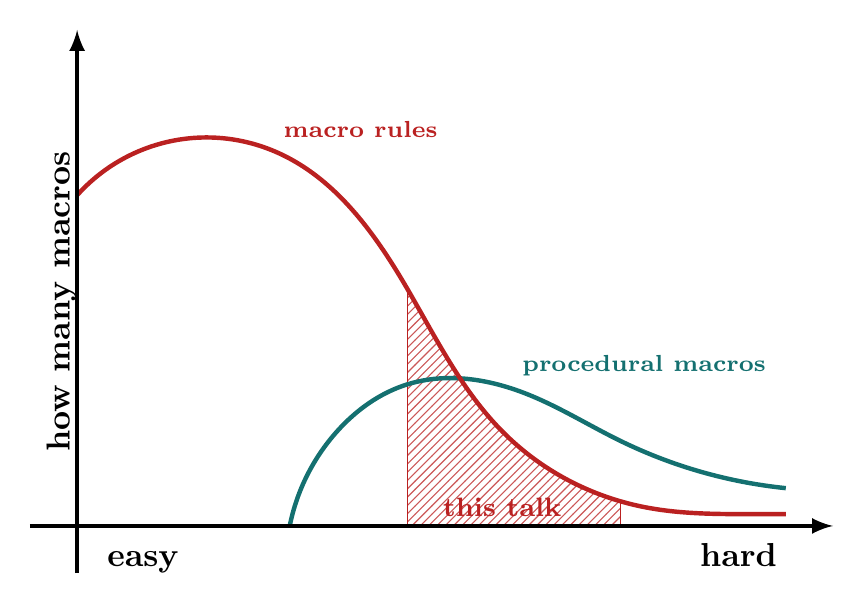
\begin{tikzpicture}[scale=1.2, every node/.style={scale=1.2}]
      \begin{scope}
        \clip[saveuse path={plot path}{
          plot[hobby]
          coordinates {(0,3.5) (2,4) (3.5,2.5) (4.5,1) (6,.2) (7,.125) (7.25,.125) (7.5,.125)}
        }] |- (0,0) -- cycle;
        \onslide<2->{
          \clip[preaction={draw,redish,pattern=north east lines,pattern color=redish!75}] (3.5,0) rectangle (5.75,5);
        }
      \end{scope}

      \onslide<4->{
        \draw[tealish,ultra thick,mark=none] plot[hobby]
          coordinates {(2.25,0) (2.75,1) (3.5,1.5) (4.75,1.4) (5.75,.9) (7.5,.4)};
      }

      \draw[redish,ultra thick,mark=none,plot path];

      \draw[-latex,ultra thick]
        (0,-.5)
        -- node[left,rotate=90,anchor=south,outer sep=-3pt] {\textbf{how many macros}} (0,5.25);

      \draw[-latex,ultra thick]
        (-.5,0)
        -- (.7,0) node[below,outer sep=9pt] {\smash{\textbf{easy}}}
        -- (7,0) node[below,outer sep=9pt] {\smash{\textbf{hard}}}
        -- (8,0);

      \onslide<2->{
        \draw (4.5,.2) node[redish] {\textbf{\textsc{\footnotesize this talk}}};
      }
      \onslide<3->{
        \draw (3,4.2) node[redish] {\textbf{\scriptsize macro rules}};
      }
      \onslide<4->{
        \draw (6,1.7) node[tealish] {\textbf{\scriptsize procedural macros}};
      }
    \end{tikzpicture}
  \end{center}
  \vspace{-25pt}
\end{frame}

\begin{frame}[fragile]
  \begin{minted}{rusty}
    ~\keywordthick{let}~ response = ~\thick{json!(}~{
        ~\quot{status}~: ~\quot{error}~,
        ~\quot{retry}~: ~\keyword{false}~,
        ~\quot{message}~: ~\quot{File not found.}~
    }~\thick{)}~;
  \end{minted}
\end{frame}

\begin{frame}[fragile]
  \begin{minted}{rusty}
    ~\keywordthick{let}~ response = {
        ~\keywordthick{let}~ ~\keywordthick{mut}~ map = HashMap::new();
        map.insert(~\quot{status}~, ~String~(~\quot{error}~));
        map.insert(~\quot{retry}~, Boolean(~\keyword{false}~));
        map.insert(~\quot{message}~, ~String~(~\quot{File not f..     }~
        map
    };
  \end{minted}
\end{frame}

\begin{frame}[fragile]
  \begin{minted}{rusty}
    ~\keywordthick{let}~ response = ~\color{redish}\openquote\{~                                "
        \"status\": \"error\",
        \"retry\": false,
        \"message\": \"File not found.\"                             "
    ~\color{redish}\}\closequote~;
  \end{minted}
\end{frame}

\begin{frame}[fragile]
  \begin{minted}{rusty}
    ~\keywordthick{let}~ response = ~\color{redish}r#\openquote\{~
        ~\color{redish}\quot{status}: \quot{error},~
        ~\color{redish}\quot{retry}: false,~
        ~\color{redish}\quot{message}: \quot{File not found.}~
    ~\color{redish}\}\closequote#~;
  \end{minted}
\end{frame}

\begin{frame}[fragile]
  \begin{onlyenv}<+>
    \begin{minted}{rusty}
      ~\keywordthick{let}~ message = /* ... */;

      ~\keywordthick{let}~ response = ~\thick{json!(}~{
          ~\quot{status}~: ~\quot{error}~,
          ~\quot{retry}~: ~\keyword{false}~,
          ~\quot{message}~: message
      }~\thick{)}~;
    \end{minted}
  \end{onlyenv}
  \begin{onlyenv}<+>
    \begin{minted}{rusty}
      ~\keywordthick{let}~ ~\hi{message}~ = /* ... */;

      ~\keywordthick{let}~ response = ~\thick{json!(}~{
          ~\quot{status}~: ~\quot{error}~,
          ~\quot{retry}~: ~\keyword{false}~,
          ~\quot{message}~: ~\hi{message}~
      }~\thick{)}~;
    \end{minted}
  \end{onlyenv}
  \begin{onlyenv}<+>
    \begin{minted}{rusty}
      ~\keywordthick{let}~ message = /* ... */;

      ~\keywordthick{let}~ response = ~\thick{json!(}~{
          ~\quot{status}~: ~\quot{error}~,
          ~\quot{retry}~: ~\keyword{false}~,
          ~\quot{message}~: message
      }~\thick{)}~;
    \end{minted}
  \end{onlyenv}
\end{frame}

\begin{frame}[fragile]
  \begin{onlyenv}<+>
    \begin{minted}{rusty}
      ~\keywordthick{let}~ response = ~\thick{json!(}~{
          ~\quot{status}~: ~\quot{error}~,
          ~\quot{retry}~: i < max_retries,
          ~\quot{message}~: /* ... */
      }~\thick{)}~;
    \end{minted}
  \end{onlyenv}
  \begin{onlyenv}<+>
    \begin{minted}{rusty}
      ~\keywordthick{let}~ response = ~\thick{json!(}~{
          ~\quot{status}~: ~\quot{error}~,
          ~\quot{retry}~: ~\hi{i < max\_retries}~,
          ~\quot{message}~: /* ... */
      }~\thick{)}~;
    \end{minted}
  \end{onlyenv}
\end{frame}

\begin{frame}[fragile]{Sequence point}
  \setlength{\leftmargini}{50pt}
  \vspace{10pt}
  \textbf{\large Covered:}
  \begin{itemize}[label=\footnotesize\ding{212},labelsep=10pt]
  \vspace{-4pt}
  \item Invoking a macro --- \texttt{m!(...)}
  \end{itemize}
  \vspace{10pt}
  \textbf{\large Open questions:}
  \begin{itemize}[label=\footnotesize\ding{212},labelsep=10pt]
  \vspace{-4pt}
  \item What the heck is TT?
  \vspace{-4pt}
  \item Differences from C preprocessor macros
  \vspace{-4pt}
  \item Defining a macro
  \end{itemize}
\end{frame}

\begin{frame}[fragile]
  \begin{onlyenv}<+>
    \begin{minted}{rusty}
      ~\keyword{macro\_rules!}~ ~\thick{json}~ {
          (...) => { ... }
      }
      ~~
      ~~
    \end{minted}
  \end{onlyenv}
  \begin{onlyenv}<+>
    \begin{minted}{rusty}
      ~\keyword{macro\_rules!}~ ~\thick{json}~ {
          (~\hi{...}~) => { ... }
      }
      ~~
      ~~
    \end{minted}
  \end{onlyenv}
  \begin{onlyenv}<+>
    \begin{minted}{rusty}
      ~\keyword{macro\_rules!}~ ~\thick{json}~ {
          (...) => {~\hi{ ... \ }~}
      }
      ~~
      ~~
    \end{minted}
  \end{onlyenv}
  \begin{onlyenv}<+>
    \begin{minted}{rusty}
      ~\keyword{macro\_rules!}~ ~\thick{json}~ {
          (...) => { ... }

          (...) => { ... }
      }
    \end{minted}
  \end{onlyenv}
\end{frame}

\begin{frame}[fragile]
  \begin{onlyenv}<+>
    \begin{minted}{rusty}
      ~\keyword{macro\_rules!}~ ~\thick{demo}~ {
          (step1) => { ~\thick{demo!(}~step2~\thick{)}~ }
          (step2) => { ~\quot{done}~ }
      }

      ~\keywordthick{let}~ output = ~\thick{demo!(}~step1~\thick{)}~;
    \end{minted}
  \end{onlyenv}
  \begin{onlyenv}<+>
    \begin{minted}{rusty}
      ~\keyword{macro\_rules!}~ ~\thick{demo}~ {
          (~\hi{step1}~) => { ~\thick{demo!(}~step2~\thick{)}~ }
          (step2) => { ~\quot{done}~ }
      }

      ~\keywordthick{let}~ output = ~\thick{demo!(}~step1~\thick{)}~;
    \end{minted}
  \end{onlyenv}
  \begin{onlyenv}<+>
    \begin{minted}{rusty}
      ~\keyword{macro\_rules!}~ ~\thick{demo}~ {
          (step1) => { ~\thick{demo!(}~step2~\thick{)}~ }
          (~\hi{step2}~) => { ~\quot{done}~ }
      }

      ~\keywordthick{let}~ output = ~\thick{demo!(}~step1~\thick{)}~;
    \end{minted}
  \end{onlyenv}
  \begin{onlyenv}<+>
    \begin{minted}{rusty}
      ~\keyword{macro\_rules!}~ ~\thick{demo}~ {
          (step1) => { ~\thick{demo!(}~step2~\thick{)}~ }
          (step2) => { ~\quot{done}~ }
      }

      ~\keywordthick{let}~ output = ~\hi{\thick{demo!(}step1\thick{)}}~;
    \end{minted}
  \end{onlyenv}
  \begin{onlyenv}<+>
    \begin{minted}{rusty}
      ~\keyword{macro\_rules!}~ ~\thick{demo}~ {
          (step1) => { ~\thick{demo!(}~step2~\thick{)}~ }
          (step2) => { ~\quot{done}~ }
      }

      ~\keywordthick{let}~ output = ~\thick{demo!(}\hi{step1}\thick{)}~;
    \end{minted}
  \end{onlyenv}
  \begin{onlyenv}<+>
    \begin{minted}{rusty}
      ~\keyword{macro\_rules!}~ ~\thick{demo}~ {
          (~\hi{step1}~) => { ~\thick{demo!(}~step2~\thick{)}~ }
          (step2) => { ~\quot{done}~ }
      }

      ~\keywordthick{let}~ output = ~\thick{demo!(}\hi{step1}\thick{)}~;
    \end{minted}
  \end{onlyenv}
  \begin{onlyenv}<+>
    \begin{minted}{rusty}
      ~\keyword{macro\_rules!}~ ~\thick{demo}~ {
          (step1) => { ~\hi{\thick{demo!(}step2\thick{)}}~ }
          (step2) => { ~\quot{done}~ }
      }

      ~\keywordthick{let}~ output = ~\thick{demo!(}~step1~\thick{)}~;
    \end{minted}
  \end{onlyenv}
  \begin{onlyenv}<+>
    \begin{minted}{rusty}
      ~\keyword{macro\_rules!}~ ~\thick{demo}~ {
          (step1) => { ~\thick{demo!(}\hi{step2}\thick{)}~ }
          (step2) => { ~\quot{done}~ }
      }

      ~\keywordthick{let}~ output = ~\thick{demo!(}~step1~\thick{)}~;
    \end{minted}
  \end{onlyenv}
  \begin{onlyenv}<+>
    \begin{minted}{rusty}
      ~\keyword{macro\_rules!}~ ~\thick{demo}~ {
          (~\hired{step1}~) => { ~\thick{demo!(}\hi{step2}\thick{)}~ }
          (step2) => { ~\quot{done}~ }
      }

      ~\keywordthick{let}~ output = ~\thick{demo!(}~step1~\thick{)}~;
    \end{minted}
  \end{onlyenv}
  \begin{onlyenv}<+>
    \begin{minted}{rusty}
      ~\keyword{macro\_rules!}~ ~\thick{demo}~ {
          (step1) => { ~\thick{demo!(}\hi{step2}\thick{)}~ }
          (~\hi{step2}~) => { ~\quot{done}~ }
      }

      ~\keywordthick{let}~ output = ~\thick{demo!(}~step1~\thick{)}~;
    \end{minted}
  \end{onlyenv}
  \begin{onlyenv}<+>
    \begin{minted}{rusty}
      ~\keyword{macro\_rules!}~ ~\thick{demo}~ {
          (step1) => { ~\thick{demo!(}~step2~\thick{)}~ }
          (step2) => { ~\hiq{done}~ }
      }

      ~\keywordthick{let}~ output = ~\thick{demo!(}~step1~\thick{)}~;
    \end{minted}
  \end{onlyenv}
  \begin{onlyenv}<+>
    \begin{minted}{rusty}
      ~\keyword{macro\_rules!}~ ~\thick{demo}~ {
          (step1) => { ~\thick{demo!(}~step2~\thick{)}~ }
          (step2) => { ~\quot{done}~ }
      }

      ~\keywordthick{let}~ output = ~\thick{demo!(}~step1~\thick{)}~;
    \end{minted}
  \end{onlyenv}
\end{frame}

\begin{frame}[fragile]
  \begin{onlyenv}<+>
    \begin{minted}{rusty}
      ~\keyword{macro\_rules!}~ ~\thick{status\_codes}~ {
          (~\color{goldish}\thick{\dollar(}{\dollar}k:expr~ => ~\color{goldish}{\dollar}v:expr~ ,~\color{goldish}\thick{)*}~) => {
              /* ... */
          }
      }
      ~~
      ~~
      ~~
      ~~
      ~~
    \end{minted}
  \end{onlyenv}
  \begin{onlyenv}<+>
    \begin{minted}{rusty}
      ~\keyword{macro\_rules!}~ ~\thick{status\_codes}~ {
          (~\color{goldish}\thick{\dollar(}~~\hi{{\dollar}k:expr}~ => ~\color{goldish}{\dollar}v:expr~ ,~\color{goldish}\thick{)*}~) => {
              /* ... */
          }
      }
      ~~
      ~~
      ~~
      ~~
      ~~
    \end{minted}
  \end{onlyenv}
  \begin{onlyenv}<+>
    \begin{minted}{rusty}
      ~\keyword{macro\_rules!}~ ~\thick{status\_codes}~ {
          (~\color{goldish}\thick{\dollar(}{\dollar}k:expr~ => ~\hi{{\dollar}v:expr}~ ,~\color{goldish}\thick{)*}~) => {
              /* ... */
          }
      }
      ~~
      ~~
      ~~
      ~~
      ~~
    \end{minted}
  \end{onlyenv}
  \begin{onlyenv}<+>
    \begin{minted}{rusty}
      ~\keyword{macro\_rules!}~ ~\thick{status\_codes}~ {
          (~\hi{\thick{\dollar(}}\color{goldish}{\dollar}k:expr~ => ~\color{goldish}{\dollar}v:expr~ ,~\hi{\thick{)*}}~) => {
              /* ... */
          }
      }
      ~~
      ~~
      ~~
      ~~
      ~~
    \end{minted}
  \end{onlyenv}
  \begin{onlyenv}<+>
    \begin{minted}{rusty}
      ~\keyword{macro\_rules!}~ ~\thick{status\_codes}~ {
          (~\color{goldish}\thick{\dollar(}{\dollar}k:expr~ => ~\color{goldish}{\dollar}v:expr~ ,~\color{goldish}\thick{)*}~) => {
              /* ... */
          }
      }
      ~~
      ~~
      ~~
      ~~
      ~~
    \end{minted}
  \end{onlyenv}
  \begin{onlyenv}<+>
    \begin{minted}{rusty}
      ~\keyword{macro\_rules!}~ ~\thick{status\_codes}~ {
          (~\color{goldish}\thick{\dollar(}{\dollar}k:expr~ => ~\color{goldish}{\dollar}v:expr~ ,~\color{goldish}\thick{)*}~) => {
              /* ... */
          }
      }

      ~\thick{status\_codes! \{}~
          404 => ~\quot{Not Found}~,
          408 => ~\quot{Request Timeout}~,
      ~\thick{\}}~
    \end{minted}
  \end{onlyenv}
  \begin{onlyenv}<+>
    \begin{minted}{rusty}
      ~\keyword{macro\_rules!}~ ~\thick{status\_codes}~ {
          (~\hi{\thick{\dollar(}}\color{goldish}{\dollar}k:expr~ => ~\color{goldish}{\dollar}v:expr~ ,~\hi{\thick{)*}}~) => {
              /* ... */
          }
      }

      ~\thick{status\_codes! \{}~
          404 => ~\quot{Not Found}~,
          408 => ~\quot{Request Timeout}~,
      ~\thick{\}}~
    \end{minted}
  \end{onlyenv}
  \begin{onlyenv}<+>
    \begin{minted}{rusty}
      ~\keyword{macro\_rules!}~ ~\thick{status\_codes}~ {
          (~{\color{goldish}\thick{\dollar(}}\hi{{\dollar}k:expr}~ => ~\color{goldish}{\dollar}v:expr~ ,~\color{goldish}\thick{)*}~) => {
              /* ... */
          }
      }

      ~\thick{status\_codes! \{}~
          ~\hi{404}~ => ~\quot{Not Found}~,
          408 => ~\quot{Request Timeout}~,
      ~\thick{\}}~
    \end{minted}
  \end{onlyenv}
  \begin{onlyenv}<+>
    \begin{minted}{rusty}
      ~\keyword{macro\_rules!}~ ~\thick{status\_codes}~ {
          (~\color{goldish}\thick{\dollar(}{\dollar}k:expr~ ~\hi{=>}~ ~\color{goldish}{\dollar}v:expr~ ,~\color{goldish}\thick{)*}~) => {
              /* ... */
          }
      }

      ~\thick{status\_codes! \{}~
          404 ~\hi{=>}~ ~\quot{Not Found}~,
          408 => ~\quot{Request Timeout}~,
      ~\thick{\}}~
    \end{minted}
  \end{onlyenv}
  \begin{onlyenv}<+>
    \begin{minted}{rusty}
      ~\keyword{macro\_rules!}~ ~\thick{status\_codes}~ {
          (~\color{goldish}\thick{\dollar(}{\dollar}k:expr~ => ~\hi{{\dollar}v:expr}~ ,~\color{goldish}\thick{)*}~) => {
              /* ... */
          }
      }

      ~\thick{status\_codes! \{}~
          404 => ~\hiq{Not Found}~,
          408 => ~\quot{Request Timeout}~,
      ~\thick{\}}~
    \end{minted}
  \end{onlyenv}
  \begin{onlyenv}<+>
    \begin{minted}{rusty}
      ~\keyword{macro\_rules!}~ ~\thick{status\_codes}~ {
          (~\color{goldish}\thick{\dollar(}{\dollar}k:expr~ => ~\color{goldish}{\dollar}v:expr~ ~\hi{,}\color{goldish}\thick{)*}~) => {
              /* ... */
          }
      }

      ~\thick{status\_codes! \{}~
          404 => ~\quot{Not Found}\hi{,}~
          408 => ~\quot{Request Timeout}~,
      ~\thick{\}}~
    \end{minted}
  \end{onlyenv}
  \begin{onlyenv}<+>
    \begin{minted}{rusty}
      ~\keyword{macro\_rules!}~ ~\thick{status\_codes}~ {
          (~{\color{goldish}\thick{\dollar(}}\hi{{\dollar}k:expr}~ => ~\color{goldish}{\dollar}v:expr~ ,~\color{goldish}\thick{)*}~) => {
              /* ... */
          }
      }

      ~\thick{status\_codes! \{}~
          404 => ~\quot{Not Found}~,
          ~\hi{408}~ => ~\quot{Request Timeout}~,
      ~\thick{\}}~
    \end{minted}
  \end{onlyenv}
  \begin{onlyenv}<+>
    \begin{minted}{rusty}
      ~\keyword{macro\_rules!}~ ~\thick{status\_codes}~ {
          (~\color{goldish}\thick{\dollar(}{\dollar}k:expr~ ~\hi{=>}~ ~\color{goldish}{\dollar}v:expr~ ,~\color{goldish}\thick{)*}~) => {
              /* ... */
          }
      }

      ~\thick{status\_codes! \{}~
          404 => ~\quot{Not Found}~,
          408 ~\hi{=>}~ ~\quot{Request Timeout}~,
      ~\thick{\}}~
    \end{minted}
  \end{onlyenv}
  \begin{onlyenv}<+>
    \begin{minted}{rusty}
      ~\keyword{macro\_rules!}~ ~\thick{status\_codes}~ {
          (~\color{goldish}\thick{\dollar(}{\dollar}k:expr~ => ~\hi{{\dollar}v:expr}~ ,~\color{goldish}\thick{)*}~) => {
              /* ... */
          }
      }

      ~\thick{status\_codes! \{}~
          404 => ~\quot{Not Found}~,
          408 => ~\hiq{Request Timeout}~,
      ~\thick{\}}~
    \end{minted}
  \end{onlyenv}
  \begin{onlyenv}<+>
    \begin{minted}{rusty}
      ~\keyword{macro\_rules!}~ ~\thick{status\_codes}~ {
          (~\color{goldish}\thick{\dollar(}{\dollar}k:expr~ => ~\color{goldish}{\dollar}v:expr~ ~\hi{,}\color{goldish}\thick{)*}~) => {
              /* ... */
          }
      }

      ~\thick{status\_codes! \{}~
          404 => ~\quot{Not Found}~,
          408 => ~\quot{Request Timeout}\hi{,}~
      ~\thick{\}}~
    \end{minted}
  \end{onlyenv}
  \begin{onlyenv}<+>
    \begin{minted}{rusty}
      ~\keyword{macro\_rules!}~ ~\thick{status\_codes}~ {
          (~\color{goldish}\thick{\dollar(}{\dollar}k:expr~ => ~\color{goldish}{\dollar}v:expr~ ,~\color{goldish}\thick{)*}~) => {
              /* ... */
          }
      }

      ~\thick{status\_codes! \{}~
          404 => ~\quot{Not Found}~,
          408 => ~\quot{Request Timeout}~,
      ~\thick{\}}~
    \end{minted}
  \end{onlyenv}
  \begin{onlyenv}<+>
    \begin{minted}{rusty}
      ~\keyword{macro\_rules!}~ ~\thick{status\_codes}~ {
          (~\color{goldish}\thick{\dollar(}{\dollar}k:expr~ => ~\color{goldish}{\dollar}v:expr~ ,~\color{goldish}\thick{)*}~) => {
              ~\hi{\omitted}~
          }
      }

      ~\thick{status\_codes! \{}~
          404 => ~\quot{Not Found}~,
          408 => ~\quot{Request Timeout}~,
      ~\thick{\}}~
    \end{minted}
  \end{onlyenv}
  \begin{onlyenv}<+>
    \begin{minted}{rusty}
      ~\keyword{macro\_rules!}~ ~\thick{status\_codes}~ {
          (~\color{goldish}\thick{\dollar(}{\dollar}k:expr~ => ~\color{goldish}{\dollar}v:expr~ ,~\color{goldish}\thick{)*}~) => {
              /* ... */
          }
      }

      ~\thick{status\_codes! \{}~
          404 => ~\quot{Not Found}~,
          408 => ~\quot{Request Timeout}~,
      ~\thick{\}}~
    \end{minted}
  \end{onlyenv}
\end{frame}

\begin{frame}[fragile]{Sequence point}
  \setlength{\leftmargini}{50pt}
  \vspace{8pt}
  \textbf{\large Covered:}
  \begin{itemize}[label=\footnotesize\ding{212},labelsep=10pt]
  \vspace{-6pt}
  \item Macro rules
  \vspace{-6pt}
  \item Fragment variables --- \texttt{\$e:expr}
  \vspace{-6pt}
  \item Repetitions --- \texttt{\$(...)*}
  \end{itemize}
  \vspace{8pt}
  \textbf{\large Open questions:}
  \begin{itemize}[label=\footnotesize\ding{212},labelsep=10pt]
  \vspace{-6pt}
  \item What the heck is TT?
  \vspace{-6pt}
  \item Ambiguities?
  \end{itemize}
\end{frame}

\begin{frame}[fragile]
  \begin{minted}{rusty}
    ~\keywordthick{let}~ response = ~\thick{json!(}~{
        ~\quot{status}~: ~\quot{error}~,
        ~\quot{retry}~: ~\keyword{false}~,
        ~\quot{message}~: ~\quot{File not found.}~
    }~\thick{)}~;
  \end{minted}
\end{frame}

\begin{frame}[fragile]
  \begin{onlyenv}<+>
    \begin{minted}{rusty}
      ~\keyword{macro\_rules!}~ ~\thick{json}~ {
          ([ ... ]) => { ... }
          ({ ... }) => { ... }
          (~\color{goldish}{\dollar}other:expr~) => { ... }
      }
    \end{minted}
  \end{onlyenv}
  \begin{onlyenv}<+>
    \begin{minted}{rusty}
      ~\keyword{macro\_rules!}~ ~\thick{json}~ {
          (~\hi{[ ... ]}~) => { ... }
          ({ ... }) => { ... }
          (~\color{goldish}{\dollar}other:expr~) => { ... }
      }
    \end{minted}
  \end{onlyenv}
  \begin{onlyenv}<+>
    \begin{minted}{rusty}
      ~\keyword{macro\_rules!}~ ~\thick{json}~ {
          ([ ... ]) => { ... }
          (~\hi{\{ ... \}}~) => { ... }
          (~\color{goldish}{\dollar}other:expr~) => { ... }
      }
    \end{minted}
  \end{onlyenv}
  \begin{onlyenv}<+>
    \begin{minted}{rusty}
      ~\keyword{macro\_rules!}~ ~\thick{json}~ {
          ([ ... ]) => { ... }
          ({ ... }) => { ... }
          (~\hi{{\dollar}other:expr}~) => { ... }
      }
    \end{minted}
  \end{onlyenv}
  \begin{onlyenv}<+>
    \begin{minted}{rusty}
      ~\keyword{macro\_rules!}~ ~\thick{json}~ {
          ([ ... ]) => { ... }
          ({ ... }) => { ... }
          (~\color{goldish}{\dollar}other:expr~) => { ... }
      }
    \end{minted}
  \end{onlyenv}
  \begin{onlyenv}<+>
    \begin{minted}{rusty}
      ~\keyword{macro\_rules!}~ ~\thick{json}~ {
          ([~\hi{ ... \ }~]) => { ... }
          ({ ... }) => { ... }
          (~\color{goldish}{\dollar}other:expr~) => { ... }
      }
    \end{minted}
  \end{onlyenv}
\end{frame}

\begin{frame}[fragile]
  \begin{onlyenv}<+>
    \begin{minted}{rusty}
      ~\thick{json!(}~[1, {~\quot{k}~: ~\quot{v}~}, i < retries]~\thick{)}~
      ~~
      ~~
      ~~
      ~~
      ~~
      ~~
      ~~
    \end{minted}
  \end{onlyenv}
  \begin{onlyenv}<+>
    \begin{minted}{rusty}
      ~\thick{json!(}~[~\hi{1}~, {~\quot{k}~: ~\quot{v}~}, i < retries]~\thick{)}~
      ~~
      ~~
      ~~
      ~~
      ~~
      ~~
      ~~
    \end{minted}
  \end{onlyenv}
  \begin{onlyenv}<+>
    \begin{minted}{rusty}
      ~\thick{json!(}~[1, ~\hi{\{\blackquote{k}: \blackquote{v}\}}~, i < retries]~\thick{)}~
      ~~
      ~~
      ~~
      ~~
      ~~
      ~~
      ~~
    \end{minted}
  \end{onlyenv}
  \begin{onlyenv}<+>
    \begin{minted}{rusty}
      ~\thick{json!(}~[1, {~\quot{k}~: ~\quot{v}~}, ~\hi{i < retries}~]~\thick{)}~
      ~~
      ~~
      ~~
      ~~
      ~~
      ~~
      ~~
    \end{minted}
  \end{onlyenv}
  \begin{onlyenv}<+>
    \begin{minted}{rusty}
      ~\thick{json!(}~[1, {~\quot{k}~: ~\quot{v}~}, i < retries]~\thick{)}~

      ~\keyword{macro\_rules!}~ ~\thick{json}~ {
          ([ ~\hi{???}~ ]) => { ... }
          // other rules
      }
      ~~
      ~~
    \end{minted}
  \end{onlyenv}
  \begin{onlyenv}<+>
    \begin{minted}{rusty}
      ~\thick{json!(}~[1, {~\quot{k}~: ~\quot{v}~}, i < retries]~\thick{)}~

      ~\keyword{macro\_rules!}~ ~\thick{json}~ {
          ([ ~{\color{goldish}\thick{\dollar(}}\hi{{\dollar}e:expr}~ ,~\color{goldish}\thick{)*}~ ]) => { ... }
          // other rules
      }
      ~~
      ~~
    \end{minted}
  \end{onlyenv}
  \begin{onlyenv}<+>
    \begin{minted}{rusty}
      ~\thick{json!(}~[1, ~\hi{\{\blackquote{k}: \blackquote{v}\}}~, i < retries]~\thick{)}~

      ~\keyword{macro\_rules!}~ ~\thick{json}~ {
          ([ ~\color{goldish}\thick{\dollar(}{\dollar}e:expr~ ,~\color{goldish}\thick{)*}~ ]) => { ... }
          // other rules
      }
      ~~
      ~~
    \end{minted}
  \end{onlyenv}
  \begin{onlyenv}<+>
    \begin{minted}{rusty}
      ~\thick{json!(}~[1, {~\quot{k}~: ~\quot{v}~}, i < retries]~\thick{)}~

      ~\keyword{macro\_rules!}~ ~\thick{json}~ {
          ([ ~\color{goldish}\thick{\dollar(}{\dollar}e:expr~ ,~\color{goldish}\thick{)*}~ ]) => { ... }
          // other rules
      }
      ~~
      ~~
    \end{minted}
  \end{onlyenv}
  \begin{onlyenv}<+>
    \begin{minted}{rusty}
      ~\thick{json!(}~[1, {~\quot{k}~: ~\quot{v}~}, i < retries]~\thick{)}~

      ~\keyword{macro\_rules!}~ ~\thick{json}~ {
          ([ ~\color{goldish}\thick{\dollar(}~~\hi{[...] OR \{...\} OR {\dollar}expr}~,~\color{goldish}\thick{)*}~ ]) => {
              ...
          }
          // other rules
      }
    \end{minted}
  \end{onlyenv}
  \begin{onlyenv}<+>
    \begin{minted}{rusty}
      ~\thick{json!(}~[1, {~\quot{k}~: ~\quot{v}~}, i < retries]~\thick{)}~

      ~\keyword{macro\_rules!}~ ~\thick{json}~ {
          ([ ~\color{goldish}\thick{\dollar(}~[...] OR {...} OR ~\color{goldish}{\dollar}expr~,~\color{goldish}\thick{)*}~ ]) => {
              ...
          }
          // other rules
      }
    \end{minted}
  \end{onlyenv}
  \begin{onlyenv}<+>
    \begin{minted}{rusty}
      ~\thick{json!(}~[1, {~\quot{k}~: ~\quot{v}~}, i < retries]~\thick{)}~

      ~\keyword{macro\_rules!}~ ~\thick{json}~ {
          ([ ~\color{goldish}\thick{\dollar(}~ [...] ,~\color{goldish}\thick{)*}~ ]) => { ... }
          ([ ~\color{goldish}\thick{\dollar(}~ {...} ,~\color{goldish}\thick{)*}~ ]) => { ... }
          ([ ~\color{goldish}\thick{\dollar(} {\dollar}e:expr~ ,~\color{goldish}\thick{)*}~ ]) => { ... }
          // other rules
      }
    \end{minted}
  \end{onlyenv}
  \begin{onlyenv}<+>
    \begin{minted}{rusty}
      ~\thick{json!(}~[1, {~\quot{k}~: ~\quot{v}~}, i < retries]~\thick{)}~

      ~\keyword{macro\_rules!}~ ~\thick{json}~ {
          (~\hi{[ \thick{\dollar(} [...] ,\thick{)*} ]}~) => { ... }
          ([ ~\color{goldish}\thick{\dollar(}~ {...} ,~\color{goldish}\thick{)*}~ ]) => { ... }
          ([ ~\color{goldish}\thick{\dollar(} {\dollar}e:expr~ ,~\color{goldish}\thick{)*}~ ]) => { ... }
          // other rules
      }
    \end{minted}
  \end{onlyenv}
  \begin{onlyenv}<+>
    \begin{minted}{rusty}
      ~\thick{json!(}~[1, {~\quot{k}~: ~\quot{v}~}, i < retries]~\thick{)}~

      ~\keyword{macro\_rules!}~ ~\thick{json}~ {
          ([ ~\color{goldish}\thick{\dollar(}~ [...] ,~\color{goldish}\thick{)*}~ ]) => { ... }
          (~\hi{[ \thick{\dollar(} \{...\} ,\thick{)*} ]}~) => { ... }
          ([ ~\color{goldish}\thick{\dollar(} {\dollar}e:expr~ ,~\color{goldish}\thick{)*}~ ]) => { ... }
          // other rules
      }
    \end{minted}
  \end{onlyenv}
  \begin{onlyenv}<+>
    \begin{minted}{rusty}
      ~\thick{json!(}~[1, {~\quot{k}~: ~\quot{v}~}, i < retries]~\thick{)}~

      ~\keyword{macro\_rules!}~ ~\thick{json}~ {
          ([ ~\color{goldish}\thick{\dollar(}~ [...] ,~\color{goldish}\thick{)*}~ ]) => { ... }
          ([ ~\color{goldish}\thick{\dollar(}~ {...} ,~\color{goldish}\thick{)*}~ ]) => { ... }
          (~\hi{[ \thick{\dollar(} {\dollar}e:expr ,\thick{)*} ]}~) => { ... }
          // other rules
      }
    \end{minted}
  \end{onlyenv}
  \begin{onlyenv}<+>
    \begin{minted}{rusty}
      ~\thick{json!(}~[1, {~\quot{k}~: ~\quot{v}~}, i < retries]~\thick{)}~

      ~\keyword{macro\_rules!}~ ~\thick{json}~ {
          ([ ~\color{goldish}\thick{\dollar(}~ [...] ,~\color{goldish}\thick{)*}~ ]) => { ... }
          ([ ~\color{goldish}\thick{\dollar(}~ {...} ,~\color{goldish}\thick{)*}~ ]) => { ... }
          ([ ~\color{goldish}\thick{\dollar(} {\dollar}e:expr~ ,~\color{goldish}\thick{)*}~ ]) => { ... }
          // other rules
      }
    \end{minted}
  \end{onlyenv}
\end{frame}

\plain{What is going wrong?}

\begin{frame}[fragile]{What is going wrong?}
  \begin{itemize}[label=\footnotesize\ding{212},labelsep=10pt]
  \item \mbox{Macro rules optimize for Rust-like grammars\hspace*{-1000pt}}
  \vspace{4pt}
  \item Decision:
    \begin{itemize}[label=$\circ$,labelsep=10pt]
    \vspace{-4pt}
    \item Make the input more like Rust, \ or
    \vspace{-4pt}
    \item Power through
    \end{itemize}
  \end{itemize} 
\end{frame}

\begin{frame}[fragile]
  \begin{onlyenv}<+>
    \begin{minted}{rusty}
      ~\keywordthick{let}~ response = ~\thick{json\_map!(}~
          ~\quot{status}~ => ~\quot{error}~,
          ~\quot{cause}~ => json::NULL,
          ~\quot{backtrace}~ => ~\thick{json\_array!(}~
              ~\quot{failure::begin\_unwind}~,
              ~\quot{option::Option<T>::unwrap}~,
              ~\quot{request::Request<S>::create}~
          ~\thick{)}~,
      ~\thick{)}~;
    \end{minted}
  \end{onlyenv}
  \begin{onlyenv}<+>
    \begin{minted}{rusty}
      ~\keywordthick{let}~ response = ~\thick{json\_map!(}~
          ~\quot{status}~ ~\hi{=>}~ ~\quot{error}~,
          ~\quot{cause}~ ~\hi{=>}~ json::NULL,
          ~\quot{backtrace}~ ~\hi{=>}~ ~\thick{json\_array!(}~
              ~\quot{failure::begin\_unwind}~,
              ~\quot{option::Option<T>::unwrap}~,
              ~\quot{request::Request<S>::create}~
          ~\thick{)}~,
      ~\thick{)}~;
    \end{minted}
  \end{onlyenv}
  \begin{onlyenv}<+>
    \begin{minted}{rusty}
      ~\keywordthick{let}~ response = ~\thick{json\_map!(}~
          ~\quot{status}~ => ~\quot{error}~,
          ~\quot{cause}~ => json::NULL,
          ~\quot{backtrace}~ => ~\hi{\thick{json\_array!}}\thick{(}~
              ~\quot{failure::begin\_unwind}~,
              ~\quot{option::Option<T>::unwrap}~,
              ~\quot{request::Request<S>::create}~
          ~\thick{)}~,
      ~\thick{)}~;
    \end{minted}
  \end{onlyenv}
  \begin{onlyenv}<+>
    \begin{minted}{rusty}
      ~\keywordthick{let}~ response = ~\hi{\thick{json\_map!}}\thick{(}~
          ~\quot{status}~ => ~\quot{error}~,
          ~\quot{cause}~ => json::NULL,
          ~\quot{backtrace}~ => ~\hi{\thick{json\_array!}}\thick{(}~
              ~\quot{failure::begin\_unwind}~,
              ~\quot{option::Option<T>::unwrap}~,
              ~\quot{request::Request<S>::create}~
          ~\thick{)}~,
      ~\thick{)}~;
    \end{minted}
  \end{onlyenv}
  \begin{onlyenv}<+>
    \begin{minted}{rusty}
      ~\keywordthick{let}~ response = ~\thick{json\_map!(}~
          ~\quot{status}~ => ~\quot{error}~,
          ~\quot{cause}~ => ~\hi{json::NULL}~,
          ~\quot{backtrace}~ => ~\thick{json\_array!(}~
              ~\quot{failure::begin\_unwind}~,
              ~\quot{option::Option<T>::unwrap}~,
              ~\quot{request::Request<S>::create}~
          ~\thick{)}~,
      ~\thick{)}~;
    \end{minted}
  \end{onlyenv}
  \begin{onlyenv}<+>
    \begin{minted}{rusty}
      ~\keywordthick{let}~ response = ~\thick{json\_map!(}~
          ~\quot{status}~ => ~\quot{error}~,
          ~\quot{cause}~ => json::NULL,
          ~\quot{backtrace}~ => ~\thick{json\_array!(}~
              ~\quot{failure::begin\_unwind}~,
              ~\quot{option::Option<T>::unwrap}~,
              ~\quot{request::Request<S>::create}~
          ~\thick{)}~,
      ~\thick{)}~;
    \end{minted}
  \end{onlyenv}
\end{frame}

\begin{frame}[fragile]
  \begin{minted}{rusty}
    ~\keywordthick{let}~ response = ~\thick{json!(}~{
        ~\quot{status}~: ~\quot{error}~,
        ~\quot{cause}~: null,
        ~\quot{backtrace}~: [
            ~\quot{failure::begin\_unwind}~,
            ~\quot{option::Option<T>::unwrap}~,
            ~\quot{request::Request<S>::create}~
        ]
    }~\thick{)}~;
  \end{minted}
\end{frame}

\begin{frame}[fragile]
  \begin{onlyenv}<+>
    \begin{minted}{rusty}
      ~\thick{json!(}~[1, {~\quot{k}~: ~\quot{v}~}, i < retries]~\thick{)}~

      ~\keyword{macro\_rules!}~ ~\thick{json}~ {
          ([ ~\hi{???}~ ]) => { ... }
          // other rules
      }
    \end{minted}
  \end{onlyenv}
  \begin{onlyenv}<+>
    \begin{minted}{rusty}
      ~\thick{json!(}~[1, {~\quot{k}~: ~\quot{v}~}, i < retries]~\thick{)}~

      ~\keyword{macro\_rules!}~ ~\thick{json}~ {
          ([ ~{\color{goldish}\thick{\dollar(}}\hi{{\dollar}content:tt}\color{goldish}\thick{)*}~ ]) => { ... }
          // other rules
      }
    \end{minted}
  \end{onlyenv}
  \begin{onlyenv}<+>
    \begin{minted}{rusty}
      ~\thick{json!(}~[1, {~\quot{k}~: ~\quot{v}~}, i < retries]~\thick{)}~

      ~\keyword{macro\_rules!}~ ~\thick{json}~ {
          (~\hi{[}~ ~\color{goldish}\thick{\dollar(}{\dollar}content:tt\thick{)*}~ ~\hi{]}~) => { ... }
          // other rules
      }
    \end{minted}
  \end{onlyenv}
  \begin{onlyenv}<+>
    \begin{minted}{rusty}
      ~\thick{json!(}~[1, {~\quot{k}~: ~\quot{v}~}, i < retries]~\thick{)}~

      ~\keyword{macro\_rules!}~ ~\thick{json}~ {
          ([ ~\hi{\thick{\dollar(}}{\color{goldish}{\dollar}content:tt}\hi{\thick{)*}}~ ]) => { ... }
          // other rules
      }
    \end{minted}
  \end{onlyenv}
  \begin{onlyenv}<+>
    \begin{minted}{rusty}
      ~\thick{json!(}~[1, {~\quot{k}~: ~\quot{v}~}, i < retries]~\thick{)}~

      ~\keyword{macro\_rules!}~ ~\thick{json}~ {
          ([ ~{\color{goldish}\thick{\dollar(}}\hi{{\dollar}content:tt}\color{goldish}\thick{)*}~ ]) => { ... }
          // other rules
      }
    \end{minted}
  \end{onlyenv}
  \begin{onlyenv}<+>
    \smash{\rlap{\raisebox{-24pt}{\color{goldish}$
      \hspace{55pt}\underbracket{\hspace{9pt}}_{\color{goldish}\texttt{1}}
    $}}}
    \vspace{-20.5pt}
    \begin{minted}{rusty}
      ~\thick{json!(}~[~\hi{1}~, {~\quot{k}~: ~\quot{v}~}, i < retries]~\thick{)}~

      ~\keyword{macro\_rules!}~ ~\thick{json}~ {
          ([ ~\color{goldish}\thick{\dollar(}{\dollar}content:tt\thick{)*}~ ]) => { ... }
          // other rules
      }
    \end{minted}
  \end{onlyenv}
  \begin{onlyenv}<+>
    \smash{\rlap{\raisebox{-24pt}{\color{goldish}$
      \hspace{55pt}\underbracket{\hspace{9pt}}_{\color{goldish}\texttt{1}}
      \hspace{-1pt}\underbracket{\hspace{9pt}}_{\color{goldish}\texttt{2}}
    $}}}
    \vspace{-20.5pt}
    \begin{minted}{rusty}
      ~\thick{json!(}~[1~\hi{,}~ {~\quot{k}~: ~\quot{v}~}, i < retries]~\thick{)}~

      ~\keyword{macro\_rules!}~ ~\thick{json}~ {
          ([ ~\color{goldish}\thick{\dollar(}{\dollar}content:tt\thick{)*}~ ]) => { ... }
          // other rules
      }
    \end{minted}
  \end{onlyenv}
  \begin{onlyenv}<+>
    \smash{\rlap{\raisebox{-24pt}{\color{goldish}$
      \hspace{55pt}\underbracket{\hspace{9pt}}_{\color{goldish}\texttt{1}}
      \hspace{-1pt}\underbracket{\hspace{9pt}}_{\color{goldish}\texttt{2}}
      \hspace{6pt}\underbracket{\hspace{89pt}}_{\color{goldish}\texttt{3}}
    $}}}
    \vspace{-20.5pt}
    \begin{minted}{rusty}
      ~\thick{json!(}~[1, ~\hi{\{\blackquote{k}: \blackquote{v}\}}~, i < retries]~\thick{)}~

      ~\keyword{macro\_rules!}~ ~\thick{json}~ {
          ([ ~\color{goldish}\thick{\dollar(}{\dollar}content:tt\thick{)*}~ ]) => { ... }
          // other rules
      }
    \end{minted}
  \end{onlyenv}
  \begin{onlyenv}<+>
    \smash{\rlap{\raisebox{-24pt}{\color{goldish}$
      \hspace{55pt}\underbracket{\hspace{9pt}}_{\color{goldish}\texttt{1}}
      \hspace{-1pt}\underbracket{\hspace{9pt}}_{\color{goldish}\texttt{2}}
      \hspace{6pt}\underbracket{\hspace{89pt}}_{\color{goldish}\texttt{3}}
      \hspace{-1pt}\underbracket{\hspace{9pt}}_{\color{goldish}\texttt{4}}
    $}}}
    \vspace{-20.5pt}
    \begin{minted}{rusty}
      ~\thick{json!(}~[1, {~\quot{k}~: ~\quot{v}~}~\hi{,}~ i < retries]~\thick{)}~

      ~\keyword{macro\_rules!}~ ~\thick{json}~ {
          ([ ~\color{goldish}\thick{\dollar(}{\dollar}content:tt\thick{)*}~ ]) => { ... }
          // other rules
      }
    \end{minted}
  \end{onlyenv}
  \begin{onlyenv}<+>
    \smash{\rlap{\raisebox{-24pt}{\color{goldish}$
      \hspace{55pt}\underbracket{\hspace{9pt}}_{\color{goldish}\texttt{1}}
      \hspace{-1pt}\underbracket{\hspace{9pt}}_{\color{goldish}\texttt{2}}
      \hspace{6pt}\underbracket{\hspace{89pt}}_{\color{goldish}\texttt{3}}
      \hspace{-1pt}\underbracket{\hspace{9pt}}_{\color{goldish}\texttt{4}}
      \hspace{6.5pt}\underbracket{\hspace{9pt}}_{\color{goldish}\texttt{5}}
    $}}}
    \vspace{-20.5pt}
    \begin{minted}{rusty}
      ~\thick{json!(}~[1, {~\quot{k}~: ~\quot{v}~}, ~\hi{i}~ < retries]~\thick{)}~

      ~\keyword{macro\_rules!}~ ~\thick{json}~ {
          ([ ~\color{goldish}\thick{\dollar(}{\dollar}content:tt\thick{)*}~ ]) => { ... }
          // other rules
      }
    \end{minted}
  \end{onlyenv}
  \begin{onlyenv}<+>
    \smash{\rlap{\raisebox{-24pt}{\color{goldish}$
      \hspace{55pt}\underbracket{\hspace{9pt}}_{\color{goldish}\texttt{1}}
      \hspace{-1pt}\underbracket{\hspace{9pt}}_{\color{goldish}\texttt{2}}
      \hspace{6pt}\underbracket{\hspace{89pt}}_{\color{goldish}\texttt{3}}
      \hspace{-1pt}\underbracket{\hspace{9pt}}_{\color{goldish}\texttt{4}}
      \hspace{6.5pt}\underbracket{\hspace{9pt}}_{\color{goldish}\texttt{5}}
      \hspace{6.5pt}\underbracket{\hspace{9pt}}_{\color{goldish}\texttt{6}}
    $}}}
    \vspace{-20.5pt}
    \begin{minted}{rusty}
      ~\thick{json!(}~[1, {~\quot{k}~: ~\quot{v}~}, i ~\hi{<}~ retries]~\thick{)}~

      ~\keyword{macro\_rules!}~ ~\thick{json}~ {
          ([ ~\color{goldish}\thick{\dollar(}{\dollar}content:tt\thick{)*}~ ]) => { ... }
          // other rules
      }
    \end{minted}
  \end{onlyenv}
  \begin{onlyenv}<+>
    \smash{\rlap{\raisebox{-24pt}{\color{goldish}$
      \hspace{55pt}\underbracket{\hspace{9pt}}_{\color{goldish}\texttt{1}}
      \hspace{-1pt}\underbracket{\hspace{9pt}}_{\color{goldish}\texttt{2}}
      \hspace{6pt}\underbracket{\hspace{89pt}}_{\color{goldish}\texttt{3}}
      \hspace{-1pt}\underbracket{\hspace{9pt}}_{\color{goldish}\texttt{4}}
      \hspace{6.5pt}\underbracket{\hspace{9pt}}_{\color{goldish}\texttt{5}}
      \hspace{6.5pt}\underbracket{\hspace{9pt}}_{\color{goldish}\texttt{6}}
      \hspace{6.5pt}\underbracket{\hspace{62pt}}_{\color{goldish}\texttt{7}}
    $}}}
    \vspace{-20.5pt}
    \begin{minted}{rusty}
      ~\thick{json!(}~[1, {~\quot{k}~: ~\quot{v}~}, i < ~\hi{retries}~]~\thick{)}~

      ~\keyword{macro\_rules!}~ ~\thick{json}~ {
          ([ ~\color{goldish}\thick{\dollar(}{\dollar}content:tt\thick{)*}~ ]) => { ... }
          // other rules
      }
    \end{minted}
  \end{onlyenv}
  \begin{onlyenv}<+>
    \smash{\rlap{\raisebox{-24pt}{\color{goldish}$
      \hspace{55pt}\underbracket{\hspace{9pt}}_{\color{goldish}\texttt{1}}
      \hspace{-1pt}\underbracket{\hspace{9pt}}_{\color{goldish}\texttt{2}}
      \hspace{6pt}\underbracket{\hspace{89pt}}_{\color{goldish}\texttt{3}}
      \hspace{-1pt}\underbracket{\hspace{9pt}}_{\color{goldish}\texttt{4}}
      \hspace{6.5pt}\underbracket{\hspace{9pt}}_{\color{goldish}\texttt{5}}
      \hspace{6.5pt}\underbracket{\hspace{9pt}}_{\color{goldish}\texttt{6}}
      \hspace{6.5pt}\underbracket{\hspace{62pt}}_{\color{goldish}\texttt{7}}
    $}}}
    \vspace{-20.5pt}
    \begin{minted}{rusty}
      ~\thick{json!(}~[1, {~\quot{k}~: ~\quot{v}~}, i < retries]~\thick{)}~

      ~\keyword{macro\_rules!}~ ~\thick{json}~ {
          ([ ~\color{goldish}\thick{\dollar(}{\dollar}content:tt\thick{)*}~ ]) => { ... }
          // other rules
      }
    \end{minted}
  \end{onlyenv}
\end{frame}

\begin{frame}[fragile]
  \begin{onlyenv}<+>
    \begin{minted}{rusty}
      ~\keyword{macro\_rules!}~ ~\thick{json}~ {
          ([ ~\hi{\thick{\dollar(}{\dollar}content:tt\thick{)*}}~ ]) => {
              validate_array!(~\color{goldish}\thick{\dollar(}{\dollar}content\thick{)*}~);
          }
          // other rules
      }
    \end{minted}
  \end{onlyenv}
  \begin{onlyenv}<+>
    \begin{minted}{rusty}
      ~\keyword{macro\_rules!}~ ~\thick{json}~ {
          ([ ~\color{goldish}\thick{\dollar(}{\dollar}content:tt\thick{)*}~ ]) => {
              ~\hi{validate\_array!}~(~\color{goldish}\thick{\dollar(}{\dollar}content\thick{)*}~);
          }
          // other rules
      }
    \end{minted}
  \end{onlyenv}
  \begin{onlyenv}<+>
    \begin{minted}{rusty}
      ~\keyword{macro\_rules!}~ ~\thick{json}~ {
          (~\hi{[}~ ~\color{goldish}\thick{\dollar(}{\dollar}content:tt\thick{)*}~ ~\hi{]}~) => {
              validate_array!(~\color{goldish}\thick{\dollar(}{\dollar}content\thick{)*}~);
          }
          // other rules
      }
    \end{minted}
  \end{onlyenv}
  \begin{onlyenv}<+>
    \begin{minted}{rusty}
      ~\keyword{macro\_rules!}~ ~\thick{json}~ {
          ([ ~\hi{\thick{\dollar(}{\dollar}content:tt\thick{)*}}~ ]) => {
              validate_array!(~\hi{\thick{\dollar(}{\dollar}content\thick{)*}}~);
          }
          // other rules
      }
    \end{minted}
  \end{onlyenv}
  \begin{onlyenv}<+>
    \begin{minted}{rusty}
      ~\keyword{macro\_rules!}~ ~\thick{json}~ {
          ([ ~\color{goldish}\thick{\dollar(}{\dollar}content:tt\thick{)*}~ ]) => {
              validate_array!(~\color{goldish}\thick{\dollar(}{\dollar}content\thick{)*}~);
          }
          // other rules
      }
    \end{minted}
  \end{onlyenv}
\end{frame}

\begin{frame}[fragile]
  \begin{onlyenv}<+>
    \begin{minted}{rusty}
      ~\keyword{macro\_rules!}~ ~\thick{validate\_array}~ {
      ~~
      ~~
      ~~
      ~~
      ~~
      ~~
      ~~
      ~~
      ~~
      ~~
    \end{minted}
  \end{onlyenv}
  \begin{onlyenv}<+>
    \begin{minted}{rusty}
      ~\keyword{macro\_rules!}~ ~\thick{validate\_array}~ {
          () => {}
      ~~
      ~~
      ~~
      ~~
      ~~
      ~~
      ~~
      ~~
      ~~
    \end{minted}
  \end{onlyenv}
  \begin{onlyenv}<+>
    \begin{minted}{rusty}
      ~\keyword{macro\_rules!}~ ~\thick{validate\_array}~ {
          () => {}
          ([ ~\color{goldish}\thick{\dollar(}{\dollar}c:tt\thick{)*}~ ], ~\color{goldish}\thick{\dollar(}{\dollar}rest:tt\thick{)*}~) => {
              validate_array!(~\color{goldish}\thick{\dollar(}{\dollar}c\thick{)*}~);
              validate_array!(~\color{goldish}\thick{\dollar(}{\dollar}rest\thick{)*}~);
          }
      ~~
      ~~
      ~~
      ~~
      ~~
    \end{minted}
  \end{onlyenv}
  \begin{onlyenv}<+>
    \begin{minted}{rusty}
      ~\keyword{macro\_rules!}~ ~\thick{validate\_array}~ {
          () => {}
          (~\hi{[ \thick{\dollar(}{\dollar}c:tt\thick{)*} ]}~, ~\color{goldish}\thick{\dollar(}{\dollar}rest:tt\thick{)*}~) => {
              validate_array!(~\color{goldish}\thick{\dollar(}{\dollar}c\thick{)*}~);
              validate_array!(~\color{goldish}\thick{\dollar(}{\dollar}rest\thick{)*}~);
          }
      ~~
      ~~
      ~~
      ~~
      ~~
    \end{minted}
  \end{onlyenv}
  \begin{onlyenv}<+>
    \begin{minted}{rusty}
      ~\keyword{macro\_rules!}~ ~\thick{validate\_array}~ {
          () => {}
          ([ ~\hi{\thick{\dollar(}{\dollar}c:tt\thick{)*}}~ ], ~\color{goldish}\thick{\dollar(}{\dollar}rest:tt\thick{)*}~) => {
              validate_array!(~\color{goldish}\thick{\dollar(}{\dollar}c\thick{)*}~);
              validate_array!(~\color{goldish}\thick{\dollar(}{\dollar}rest\thick{)*}~);
          }
      ~~
      ~~
      ~~
      ~~
      ~~
    \end{minted}
  \end{onlyenv}
  \begin{onlyenv}<+>
    \begin{minted}{rusty}
      ~\keyword{macro\_rules!}~ ~\thick{validate\_array}~ {
          () => {}
          ([ ~\color{goldish}\thick{\dollar(}{\dollar}c:tt\thick{)*}~ ]~\hi{,}~ ~\color{goldish}\thick{\dollar(}{\dollar}rest:tt\thick{)*}~) => {
              validate_array!(~\color{goldish}\thick{\dollar(}{\dollar}c\thick{)*}~);
              validate_array!(~\color{goldish}\thick{\dollar(}{\dollar}rest\thick{)*}~);
          }
      ~~
      ~~
      ~~
      ~~
      ~~
    \end{minted}
  \end{onlyenv}
  \begin{onlyenv}<+>
    \begin{minted}{rusty}
      ~\keyword{macro\_rules!}~ ~\thick{validate\_array}~ {
          () => {}
          ([ ~\color{goldish}\thick{\dollar(}{\dollar}c:tt\thick{)*}~ ], ~\hi{\thick{\dollar(}{\dollar}rest:tt\thick{)*}}~) => {
              validate_array!(~\color{goldish}\thick{\dollar(}{\dollar}c\thick{)*}~);
              validate_array!(~\color{goldish}\thick{\dollar(}{\dollar}rest\thick{)*}~);
          }
      ~~
      ~~
      ~~
      ~~
      ~~
    \end{minted}
  \end{onlyenv}
  \begin{onlyenv}<+>
    \begin{minted}{rusty}
      ~\keyword{macro\_rules!}~ ~\thick{validate\_array}~ {
          () => {}
          ([ ~\hi{\thick{\dollar(}{\dollar}c:tt\thick{)*}}~ ], ~\color{goldish}\thick{\dollar(}{\dollar}rest:tt\thick{)*}~) => {
              validate_array!(~\hi{\thick{\dollar(}{\dollar}c\thick{)*}}~);
              validate_array!(~\color{goldish}\thick{\dollar(}{\dollar}rest\thick{)*}~);
          }
      ~~
      ~~
      ~~
      ~~
      ~~
    \end{minted}
  \end{onlyenv}
  \begin{onlyenv}<+>
    \begin{minted}{rusty}
      ~\keyword{macro\_rules!}~ ~\thick{validate\_array}~ {
          () => {}
          ([ ~\color{goldish}\thick{\dollar(}{\dollar}c:tt\thick{)*}~ ], ~\hi{\thick{\dollar(}{\dollar}rest:tt\thick{)*}}~) => {
              validate_array!(~\color{goldish}\thick{\dollar(}{\dollar}c\thick{)*}~);
              validate_array!(~\hi{\thick{\dollar(}{\dollar}rest\thick{)*}}~);
          }
      ~~
      ~~
      ~~
      ~~
      ~~
    \end{minted}
  \end{onlyenv}
  \begin{onlyenv}<+>
    \begin{minted}{rusty}
      ~\keyword{macro\_rules!}~ ~\thick{validate\_array}~ {
          () => {}
          ([ ~\color{goldish}\thick{\dollar(}{\dollar}c:tt\thick{)*}~ ], ~\color{goldish}\thick{\dollar(}{\dollar}rest:tt\thick{)*}~) => {
              validate_array!(~\color{goldish}\thick{\dollar(}{\dollar}c\thick{)*}~);
              validate_array!(~\color{goldish}\thick{\dollar(}{\dollar}rest\thick{)*}~);
          }
      ~~
      ~~
      ~~
      ~~
      ~~
    \end{minted}
  \end{onlyenv}
  \begin{onlyenv}<+>
    \begin{minted}{rusty}
      ~\keyword{macro\_rules!}~ ~\thick{validate\_array}~ {
          () => {}
          (~\hi{[ \thick{\dollar(}{\dollar}c:tt\thick{)*} ]}~, ~\color{goldish}\thick{\dollar(}{\dollar}rest:tt\thick{)*}~) => {
              validate_array!(~\color{goldish}\thick{\dollar(}{\dollar}c\thick{)*}~);
              validate_array!(~\color{goldish}\thick{\dollar(}{\dollar}rest\thick{)*}~);
          }
      ~~
      ~~
      ~~
      ~~
      ~~
    \end{minted}
  \end{onlyenv}
  \begin{onlyenv}<+>
    \begin{minted}{rusty}
      ~\keyword{macro\_rules!}~ ~\thick{validate\_array}~ {
          () => {}
          ([ ~\color{goldish}\thick{\dollar(}{\dollar}c:tt\thick{)*}~ ], ~\color{goldish}\thick{\dollar(}{\dollar}rest:tt\thick{)*}~) => {
              validate_array!(~\color{goldish}\thick{\dollar(}{\dollar}c\thick{)*}~);
              validate_array!(~\color{goldish}\thick{\dollar(}{\dollar}rest\thick{)*}~);
          }
          (~\hi{\{ \thick{\dollar(}{\dollar}c:tt\thick{)*} \}}~, ~\color{goldish}\thick{\dollar(}{\dollar}rest:tt\thick{)*}~) => {
              ...
          }
      ~~
      ~~
    \end{minted}
  \end{onlyenv}
  \begin{onlyenv}<+>
    \begin{minted}{rusty}
      ~\keyword{macro\_rules!}~ ~\thick{validate\_array}~ {
          () => {}
          ([ ~\color{goldish}\thick{\dollar(}{\dollar}c:tt\thick{)*}~ ], ~\color{goldish}\thick{\dollar(}{\dollar}rest:tt\thick{)*}~) => {
              validate_array!(~\color{goldish}\thick{\dollar(}{\dollar}c\thick{)*}~);
              validate_array!(~\color{goldish}\thick{\dollar(}{\dollar}rest\thick{)*}~);
          }
          ({ ~\color{goldish}\thick{\dollar(}{\dollar}c:tt\thick{)*}~ }, ~\color{goldish}\thick{\dollar(}{\dollar}rest:tt\thick{)*}~) => {
              ...
          }
      ~~
      ~~
    \end{minted}
  \end{onlyenv}
  \begin{onlyenv}<+>
    \begin{minted}{rusty}
      ~\keyword{macro\_rules!}~ ~\thick{validate\_array}~ {
          () => {}
          ([ ~\color{goldish}\thick{\dollar(}{\dollar}c:tt\thick{)*}~ ], ~\color{goldish}\thick{\dollar(}{\dollar}rest:tt\thick{)*}~) => {
              validate_array!(~\color{goldish}\thick{\dollar(}{\dollar}c\thick{)*}~);
              validate_array!(~\color{goldish}\thick{\dollar(}{\dollar}rest\thick{)*}~);
          }
          ({ ~\color{goldish}\thick{\dollar(}{\dollar}c:tt\thick{)*}~ }, ~\color{goldish}\thick{\dollar(}{\dollar}rest:tt\thick{)*}~) => {
              ...
          }
          (~\hi{{\dollar}e:expr}~, ~\color{goldish}\thick{\dollar(}{\dollar}rest:tt\thick{)*}~) => { ... }
      }
    \end{minted}
  \end{onlyenv}
  \begin{onlyenv}<+>
    \begin{minted}{rusty}
      ~\keyword{macro\_rules!}~ ~\thick{validate\_array}~ {
          () => {}
          ([ ~\color{goldish}\thick{\dollar(}{\dollar}c:tt\thick{)*}~ ], ~\color{goldish}\thick{\dollar(}{\dollar}rest:tt\thick{)*}~) => {
              validate_array!(~\color{goldish}\thick{\dollar(}{\dollar}c\thick{)*}~);
              validate_array!(~\color{goldish}\thick{\dollar(}{\dollar}rest\thick{)*}~);
          }
          ({ ~\color{goldish}\thick{\dollar(}{\dollar}c:tt\thick{)*}~ }, ~\color{goldish}\thick{\dollar(}{\dollar}rest:tt\thick{)*}~) => {
              ...
          }
          (~\color{goldish}{\dollar}e:expr~, ~\color{goldish}\thick{\dollar(}{\dollar}rest:tt\thick{)*}~) => { ... }
      }
    \end{minted}
  \end{onlyenv}
\end{frame}

\begin{frame}[fragile]
  \textbf{\large The Little Book of Rust Macros}
  {\footnotesize{\myhref{https://danielkeep.github.io/tlborm/}}}
  \setlength{\leftmargini}{50pt}
  \begin{enumerate}[labelsep=10pt]
  \item[\footnotesize\texttt{\textls*[-100]{4.}}] Patterns
  \vspace{-8pt}
    \begin{enumerate}[labelsep=10pt]
    \footnotesize
    \item[\scriptsize\texttt{\textls*[-100]{4.1}}] Callbacks
    \vspace{-4pt}
    \item[\scriptsize\texttt{\textls*[-100]{4.2}}] TT Munchers
    \vspace{-4pt}
    \item[\scriptsize\texttt{\textls*[-100]{4.3}}] Internal Rules
    \vspace{-4pt}
    \item[\scriptsize\texttt{\textls*[-100]{4.4}}] Push-Down Accumulation
    \vspace{-4pt}
    \item[\scriptsize\texttt{\textls*[-100]{4.5}}] Repetition Replacement
    \vspace{-4pt}
    \item[\scriptsize\texttt{\textls*[-100]{4.6}}] Trailing Separators
    \vspace{-4pt}
    \item[\scriptsize\texttt{\textls*[-100]{4.7}}] TT Bundling
    \end{enumerate}
  \end{enumerate}
  \vspace{-50pt}
\end{frame}

\begin{frame}[fragile]
  \begin{center}
    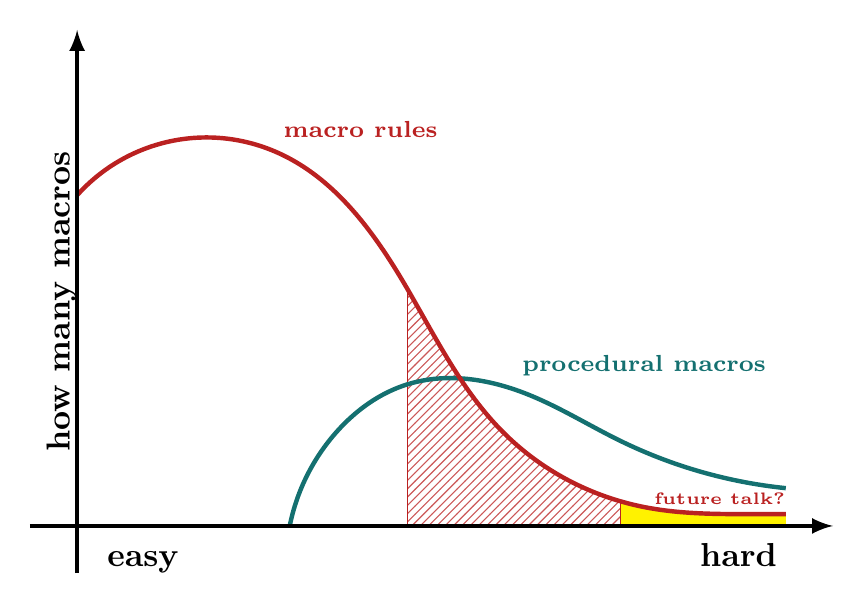
\begin{tikzpicture}[scale=1.2, every node/.style={scale=1.2}]
      \begin{scope}
        \clip[saveuse path={plot path}{
          plot[hobby]
          coordinates {(0,3.5) (2,4) (3.5,2.5) (4.5,1) (6,.2) (7,.125) (7.25,.125) (7.5,.125)}
        }] |- (0,0) -- cycle;
        \clip[preaction={fill=yellow}] (5.75,0) rectangle (7.5,5);
      \end{scope}
      \begin{scope}
        \clip[saveuse path={plot path}{
          plot[hobby]
          coordinates {(0,3.5) (2,4) (3.5,2.5) (4.5,1) (6,.2) (7,.125) (7.25,.125) (7.5,.125)}
        }] |- (0,0) -- cycle;
        \clip[preaction={draw,redish,pattern=north east lines,pattern color=redish!75}] (3.5,0) rectangle (5.75,5);
      \end{scope}

      \draw[tealish,ultra thick,mark=none] plot[hobby]
        coordinates {(2.25,0) (2.75,1) (3.5,1.5) (4.75,1.4) (5.75,.9) (7.5,.4)};

      \draw[redish,ultra thick,mark=none,plot path];

      \draw[-latex,ultra thick]
        (0,-.5)
        -- node[left,rotate=90,anchor=south,outer sep=-3pt] {\textbf{how many macros}} (0,5.25);

      \draw[-latex,ultra thick]
        (-.5,0)
        -- (.7,0) node[below,outer sep=9pt] {\smash{\textbf{easy}}}
        -- (7,0) node[below,outer sep=9pt] {\smash{\textbf{hard}}}
        -- (8,0);

      \draw (3,4.2) node[redish] {\textbf{\scriptsize macro rules}};
      \draw (6,1.7) node[tealish] {\textbf{\scriptsize procedural macros}};
      \onslide<2->{
        \draw (6.8,0.29) node[redish] {\textbf{\tiny future talk?}};
      }
    \end{tikzpicture}
  \end{center}
  \vspace{-25pt}
\end{frame}

\begin{frame}
  \begin{center}
    \myhref{https://github.com/dtolnay/tt-call}
  \end{center}
\end{frame}

\plain{}

\plain{Questions?}

\begin{frame}
\end{frame}

\begin{frame}[fragile]
  \begin{minted}{rusty}
    #![feature(trace_macros)]
    trace_macros!(~\keyword{true}~);

    ~\keyword{macro\_rules!}~ ~\thick{demo}~ {
        (step1) => { ~\thick{demo!(}~step2~\thick{)}~ }
        (step2) => { ~\quot{done}~ }
    }

    ~\keywordthick{fn}~ main() {
        ~\keywordthick{let}~ output = ~\thick{demo!(}~step1~\thick{)}~;
    }
  \end{minted}
\end{frame}

\begin{frame}[fragile]
  \begin{minted}{rusty}
    --> src/main.rs:13:18
     |
     |     ~\keywordthick{let}~ output = demo!(step1);
     |                  ^^^^^^^^^^^^
     = note: expanding ~\quotesingle{demo!(step1)}~
     = note: to ~\quotesingle{demo!(step2)}~
     = note: expanding ~\quotesingle{demo!(step2)}~
     = note: to ~\quotesingle{\quot{done}}~
  \end{minted}
\end{frame}

\begin{frame}[fragile]
  \begin{minted}{rusty}
    ~\keywordthick{enum}~ Value {
        ~Null,~
        ~Bool(bool),~
        ~Number(Number),~
        ~String(String),~
        ~Array(Vec<Value>),~
        ~Object(Map<String, Value>),~
    }
  \end{minted}
\end{frame}

\begin{frame}[fragile]
  \begin{minted}{rusty}
    ~\keyword{macro\_rules!}~ ~\thick{json}~ {
        ([ ~\color{goldish}\thick{\dollar(}{\dollar}c:tt\thick{)*}~ ]) => {
            ~\keywordthick{let}~ ~\keywordthick{mut}~ array = ~Vec~::new();
            array_helper!(array, ~\color{goldish}\thick{\dollar(}{\dollar}c\thick{)*}~);
            Value::Array(array)
        }
        // other rules
    }
  \end{minted}
\end{frame}

\begin{frame}[fragile]
  \begin{minted}{rusty}
    ~\keyword{macro\_rules!}~ ~\thick{array\_helper}~ {
        (~\color{goldish}{\dollar}a:ident~,) => {}
        (~\color{goldish}{\dollar}a:ident~, [~\color{goldish}\thick{\dollar(}{\dollar}c:tt\thick{)*}~], ~\color{goldish}\thick{\dollar(}{\dollar}r:tt\thick{)*}~) => {
            ~\color{goldish}{\dollar}a~.push(json!([~\color{goldish}\thick{\dollar(}{\dollar}c\thick{)*}~]));
            array_helper!(~\color{goldish}{\dollar}a~, ~\color{goldish}\thick{\dollar(}{\dollar}r\thick{)*}~);
        }
        // other rules
    }
  \end{minted}
\end{frame}

\begin{frame}[fragile]
  \vspace*{-8pt}
  \begin{minted}[fontsize=\footnotesize,baselinestretch=1.05]{rusty}
    ~\keyword{macro\_rules!}~ ~\thick{json}~ {
        ([ ~\color{goldish}\thick{\dollar(}{\dollar}c:tt\thick{)*}~ ]) => {
            ~\keywordthick{let}~ ~\keywordthick{mut}~ array = ~Vec~::new();
            array_helper!(array, ~\color{goldish}\thick{\dollar(}{\dollar}c\thick{)*}~);
            Value::Array(array)
        }
        // other rules
    }
    ~\keyword{macro\_rules!}~ ~\thick{array\_helper}~ {
        (~\color{goldish}{\dollar}a:ident~,) => {}
        (~\color{goldish}{\dollar}a:ident~, [~\color{goldish}\thick{\dollar(}{\dollar}c:tt\thick{)*}~], ~\color{goldish}\thick{\dollar(}{\dollar}r:tt\thick{)*}~) => {
            ~\color{goldish}{\dollar}a~.push(json!([~\color{goldish}\thick{\dollar(}{\dollar}c\thick{)*}~]));
            array_helper!(~\color{goldish}{\dollar}a~, ~\color{goldish}\thick{\dollar(}{\dollar}r\thick{)*}~);
        }
        // other rules
    }
  \end{minted}
\end{frame}

\end{document}
% vim: noai:ts=2:sw=2:tw=0
